% Generated by figures/make_figures.py from numbers.tex; do not edit.
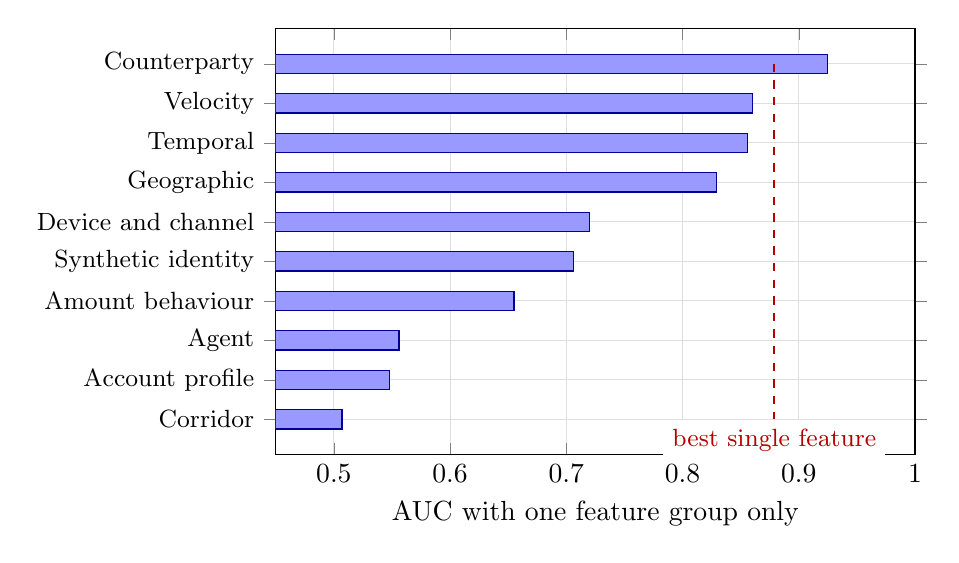
\begin{tikzpicture}
  \begin{axis}[
      width=0.8\linewidth, height=7cm,
      xbar, bar width=7pt, xmin=0.45, xmax=1.0,
      xlabel={AUC with one feature group only},
      symbolic y coords={{Counterparty},{Velocity},{Temporal},{Geographic},{Device and channel},{Synthetic identity},{Amount behaviour},{Agent},{Account profile},{Corridor}},
      ytick=data, y dir=reverse, yticklabel style={font=\small},
      grid=major, grid style={gray!25},
    ]
    \addplot[fill=blue!40, draw=blue!60!black] coordinates {(0.925,{Counterparty}) (0.86,{Velocity}) (0.856,{Temporal}) (0.829,{Geographic}) (0.72,{Device and channel}) (0.706,{Synthetic identity}) (0.655,{Amount behaviour}) (0.556,{Agent}) (0.548,{Account profile}) (0.507,{Corridor})};
    \draw[red!70!black, thick, dashed] (axis cs:0.879,{Counterparty}) -- (axis cs:0.879,{Corridor})
      node[pos=1, anchor=north, font=\small, fill=white] {best single feature};
  \end{axis}
\end{tikzpicture}
